\documentclass[dvipdfmx,aspectratio=169]{beamer}

% packages
\usepackage[deluxe]{otf}
\usepackage{pxjahyper}
\usepackage{hyperref}
\usepackage{graphicx}
\usepackage{booktabs}
\usepackage{amsmath,amssymb}
\usepackage{bm}
\usepackage{appendixnumberbeamer}

\graphicspath{{../figures/}}
\makeatletter
\def\input@path{{../tables/}}
\makeatother

\renewcommand{\kanjifamilydefault}{\gtdefault}

\uselanguage{japanese}
\languagepath{japanese}
\deftranslation[to=japanese]{Figure}{図}
\deftranslation[to=japanese]{Table}{表}
\deftranslation[to=japanese]{References}{参考文献}

% theme
\usetheme{Frankfurt}
\useinnertheme{circles}
\usefonttheme{professionalfonts}
\usecolortheme[RGB={76,114,176}]{structure}
\definecolor{deepblue}{RGB}{76,114,176}
\definecolor{deepred}{RGB}{196,78,82}

% template
\setbeamertemplate{title page}[default]
\setbeamertemplate{frametitle}[default]
\setbeamertemplate{enumerate items}[default]
\setbeamertemplate{blocks}[rounded]
\setbeamertemplate{footline}[frame number]
\setbeamertemplate{navigation symbols}{}
\setbeamertemplate{bibliography item}[text]
\setbeamerfont{footline}{size=\small}
\setbeamercolor{alerted text}{fg=deepred}

\DeclareMathOperator{\MSE}{MSE}
\DeclareMathOperator{\RMSE}{RMSE}
\DeclareMathOperator{\var}{var}
\DeclareMathOperator{\cov}{cov}
\bmdefine{\x}{x}
\newcommand{\varm}{\var(\varepsilon_\theta|\x)}
\newcommand{\varh}{\var(\varepsilon_h)}
\newcommand{\covh}{\cov(\varepsilon_h)}
\newcommand{\covmh}{\cov(\varepsilon_\theta, \varepsilon_h)}

% title
\title{A Human-Machine Ensemble Method for Economic Forecasts}
\subtitle{経済予測に関する人間と機械のアンサンブル法の考案}
\author[Takahiro MIYOSHI]{三吉 貴大}
\institute[石田・松原研究室]{社会情報ネットワーク講座・広域情報ネットワーク分野}
\date{2017年2月14日}

% サブセクションがなくても○●○を表示
\usepackage{remreset}
\makeatletter
\@removefromreset{subsection}{section}
\makeatother
\setcounter{subsection}{1}

% セクションのはじめに目次を表示
\AtBeginSection[] {
  \begin{frame}{アウトライン}
  \tableofcontents[currentsection,hideothersubsections]
  \end{frame}
}

% 1. 研究論文としての位置づけ、その分野への貢献が明確に記載されていること
% 2. 研究成果のレベルが、学術的発表(少なくとも当該学会の研究会レベル)に達していること
% 3. 研究の実施プロセスが理解できるよう記述されていること
% 4. 社会情報学との関連が議論されていること

\begin{document}

\begin{frame}[plain]
\titlepage{}
\end{frame}

\begin{frame}{アウトライン}
\tableofcontents[hideallsubsections]
\end{frame}

\section{はじめに}

\subsection{背景}

%%%%%%%%%%%%%%%%%%%%%%%%%%%%%%%%%%%%%%%%
\begin{frame}{経済予測}
\begin{block}{経済指標}
  \begin{itemize}
    \item GDPやインフレなどの経済指標は政策立案者や企業,投資家にとって重要
    \item マクロ経済モデルや時系列解析等の従来手法では,1年程度の短期予測は困難
  \end{itemize}
\end{block}
\begin{columns}[onlytextwidth]
  \begin{column}{0.48\textwidth}
    \begin{block}{集合知による予測}
      \begin{itemize}
        \item e.g. 質問紙調査の集計値
        \item 景気や政策などの情報を総合的に考慮して予測を行う
        \item 多様性を大きくすることで誤差の期待値を小さくできる~\cite{Page2008}
      \end{itemize}
    \end{block}
  \end{column}
  \begin{column}{0.48\textwidth}
    \begin{block}{機械学習による予測}
      \begin{itemize}
        \item e.g. 再帰ニューラルネット
        \item 過去の時系列から統計的に予測器を構築し予測を行う
        \item 過去のデータを元に誤差の期待値を定量化できる
      \end{itemize}
    \end{block}
  \end{column}
\end{columns}
\centering
\begin{alertblock}{}
  \centering
  \alert{これらを組み合わせて,より正確な予測を行う}
\end{alertblock}
\end{frame}
%%%%%%%%%%%%%%%%%%%%%%%%%%%%%%%%%%%%%%%%

\subsection{関連研究}

%%%%%%%%%%%%%%%%%%%%%%%%%%%%%%%%%%%%%%%%
\begin{frame}{予測の組み合わせ}
\begin{block}{アンサンブル法~\cite{Zhou2012}}
  \begin{itemize}
    \item 予測の集約には,単純平均や中央値,重み平均が一般に用いられる
    \item 重み平均では,過去の予測が正確だった予測者・予測器の重みを大きくする
    \begin{itemize}
      \item 予測者$i$の予測値を$h_i$,重みを$w_i$とすると重み平均は$\sum_i w_i h_i$
    \end{itemize}
    \item 経済予測では,必ずしもこれらの方法で予測精度が向上できるわけではない~\cite{Ang2007}
  \end{itemize}
\end{block}
\begin{alertblock}{問題}
  \begin{itemize}
    \item 入力に関わらず組み合わせ方(重み)が一定\\
          $\to$ 予測者・予測器ごとの得手不得手の違いを活かすことができない
  \end{itemize}
\end{alertblock}
\begin{alertblock}{}
  \centering
  \alert{入力に応じて,組み合わせ方を変化させる}
\end{alertblock}
\end{frame}
%%%%%%%%%%%%%%%%%%%%%%%%%%%%%%%%%%%%%%%%

\subsection{研究の目的}

%%%%%%%%%%%%%%%%%%%%%%%%%%%%%%%%%%%%%%%%
\begin{frame}{研究の目的}
\begin{columns}
  \begin{column}{0.45\textwidth}
    \begin{block}{目的}
      人間と機械の予測をうまく組み合わせることで,より正確な経済予測を行う
    \end{block}
    \begin{alertblock}{研究課題}
      \begin{enumerate}
        \item 人間と機械の予測方法の違いを反映したモデル化と,その最適な組み合わせ方の考案
        \item 考案したアンサンブル法を用いた経済予測の実装と評価
      \end{enumerate}
    \end{alertblock}
  \end{column}
  \begin{column}{0.55\textwidth}
    \begin{figure}
      \centering
      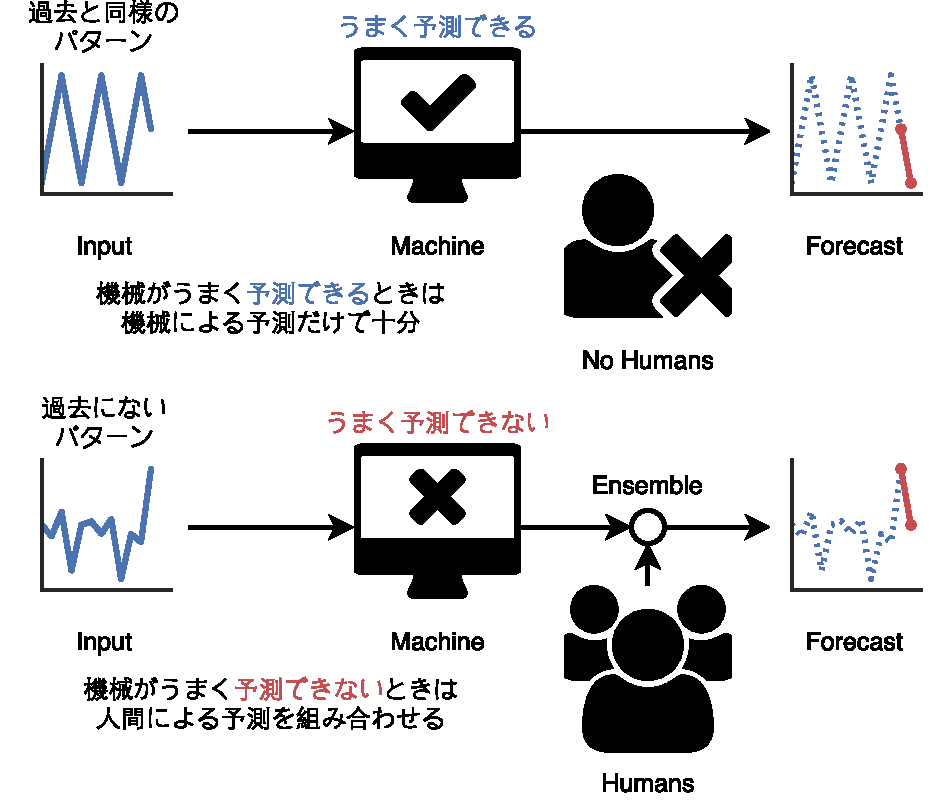
\includegraphics[width=\columnwidth]{slide-schematic.pdf}
      % \caption{提案手法の概要}
    \end{figure}
  \end{column}
\end{columns}
\end{frame}
%%%%%%%%%%%%%%%%%%%%%%%%%%%%%%%%%%%%%%%%

\section{提案手法}

\subsection{人間と機械の予測のモデル化}

%%%%%%%%%%%%%%%%%%%%%%%%%%%%%%%%%%%%%%%%
\begin{frame}{人間による予測のモデル}
  \begin{columns}
    \begin{column}{0.5\textwidth}
      \begin{block}{人間による予測のモデル~\cite{Lamberson2012}}
        予測者$i$の予測値$h_i$と誤差$\varepsilon_{h_i}$を以下のパラメータに従う確率変数とする
        \begin{itemize}
          \item $\varh$: 個人の予測の分散
          \item $\covh$: 異なる2人の誤差の共分散
          \item 予測値に偏りはないとする
        \end{itemize}
      \end{block}
      \begin{alertblock}{人間の特徴}
        \begin{itemize}
          \item 容易に人数$n$を大きくできる
          \item $\covh$が小さい$=$多様性が大きい
        \end{itemize}
      \end{alertblock}
    \end{column}
    \begin{column}{0.5\textwidth}
      \begin{figure}
        \centering
        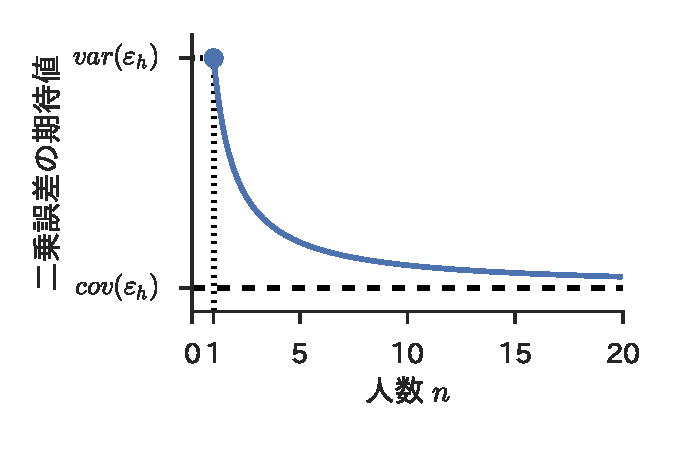
\includegraphics[width=\columnwidth]{slide-humans_graph.pdf}
        \caption{$n$人の予測の平均値における二乗誤差の期待値と人数$n$の関係.$n$を大きくするほど二乗誤差の期待値を小さくできる}
      \end{figure}
    \end{column}
  \end{columns}
\end{frame}
%%%%%%%%%%%%%%%%%%%%%%%%%%%%%%%%%%%%%%%%

%%%%%%%%%%%%%%%%%%%%%%%%%%%%%%%%%%%%%%%%
\begin{frame}{機械による予測のモデル}
  \begin{columns}
    \begin{column}{0.5\textwidth}
      \begin{block}{機械の出力として事後分布の導入}
        予測器$\theta$は入力$\x$に対して\alert{確率分布$f_\theta(y|\x)$}を出力する
        \begin{itemize}
          \item 分布の平均を予測値$y_\theta(\x)$とする
          \item 分布の分散$\varm$は二乗誤差の期待値を表す
        \end{itemize}
      \end{block}
      \begin{alertblock}{機械の特徴}
        \begin{itemize}
          \item 入力$\x$に応じた誤差の期待値をモデルに基づいて定量化できる
        \end{itemize}
      \end{alertblock}
    \end{column}
    \begin{column}{0.5\textwidth}
      \begin{figure}
        \centering
        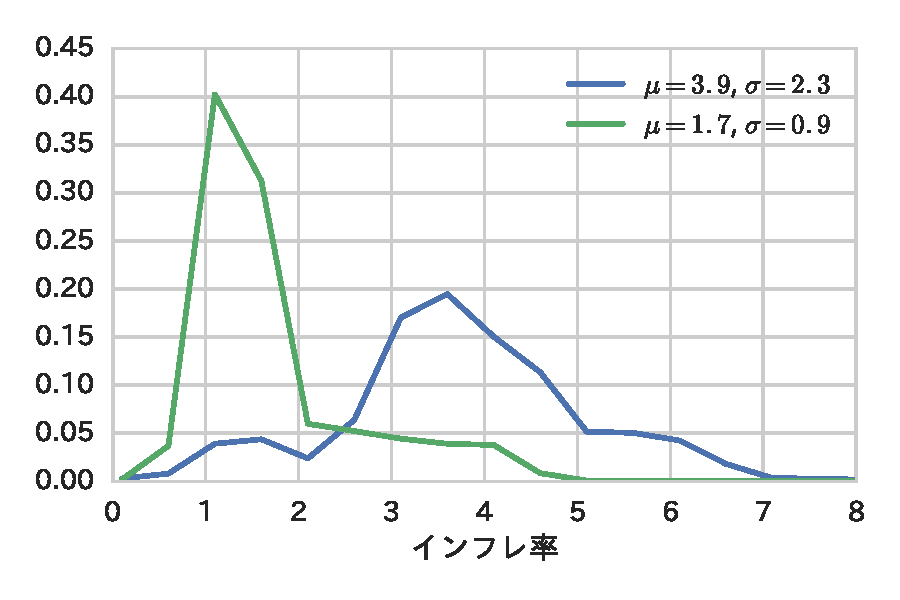
\includegraphics[width=\columnwidth]{slide-machine_outputs.pdf}
        \caption{ニューラルネットによる予測器が出力した確率分布の例.青より緑の方が分散が小さいため,誤差の期待値が小さいと考えられる}
      \end{figure}
    \end{column}
  \end{columns}
\end{frame}
%%%%%%%%%%%%%%%%%%%%%%%%%%%%%%%%%%%%%%%%

\subsection{アンサンブルの誤差の期待値の最小化}

%%%%%%%%%%%%%%%%%%%%%%%%%%%%%%%%%%%%%%%%
\begin{frame}{Human-Machine Ensemble}
\begin{alertblock}{問題の定式化}
  $n$人の人間$h_1,\dots,h_n$と一つの機械$\theta$による予測値の平均をアンサンブルの予測値$Y_{\theta,h}(n|\x)$とする
  \begin{equation}
    Y_{\theta,h}(n|\x)
      = \frac{y_\theta(\x) + \sum_{i=1}^n h_i}{n + 1}
  \end{equation}
  この\alert{二乗誤差の期待値$\MSE[Y_{\theta,h}(n|\x)]$を最小化する人数$n^\ast \geq 0$を求める}
  \begin{equation}
    \MSE[Y_{\theta,h}(n|\x)]
      = \frac{n\varh + \varm + n(n - 1)\covh + 2n\covmh}{{(n + 1)}^2}
    \label{eq: expected squared error}
  \end{equation}
  \begin{itemize}
    \item $\covmh$: 機械と人間の予測の誤差の共分散
  \end{itemize}
\end{alertblock}
\end{frame}
%%%%%%%%%%%%%%%%%%%%%%%%%%%%%%%%%%%%%%%%

%%%%%%%%%%%%%%%%%%%%%%%%%%%%%%%%%%%%%%%%
\begin{frame}{最適な人数}
\begin{columns}
  \begin{column}{0.4\textwidth}
    \begin{alertblock}{極小値を取る条件}
      式(\ref{eq: expected squared error})が極小値を持てば,最適な$n^\ast$は必ず存在する

      極小値を持つ条件は
      \begin{equation}
        \covmh < \frac{3\covh - \varh}{2}
        \label{eq: condition}
      \end{equation}
    \end{alertblock}
    \begin{block}{実用において}
      式(\ref{eq: condition})が成り立たない場合は人数の上限$N_{\text{max}}$を設定すればよい
    \end{block}
  \end{column}
  \begin{column}{0.6\textwidth}
    \begin{figure}
      \centering
      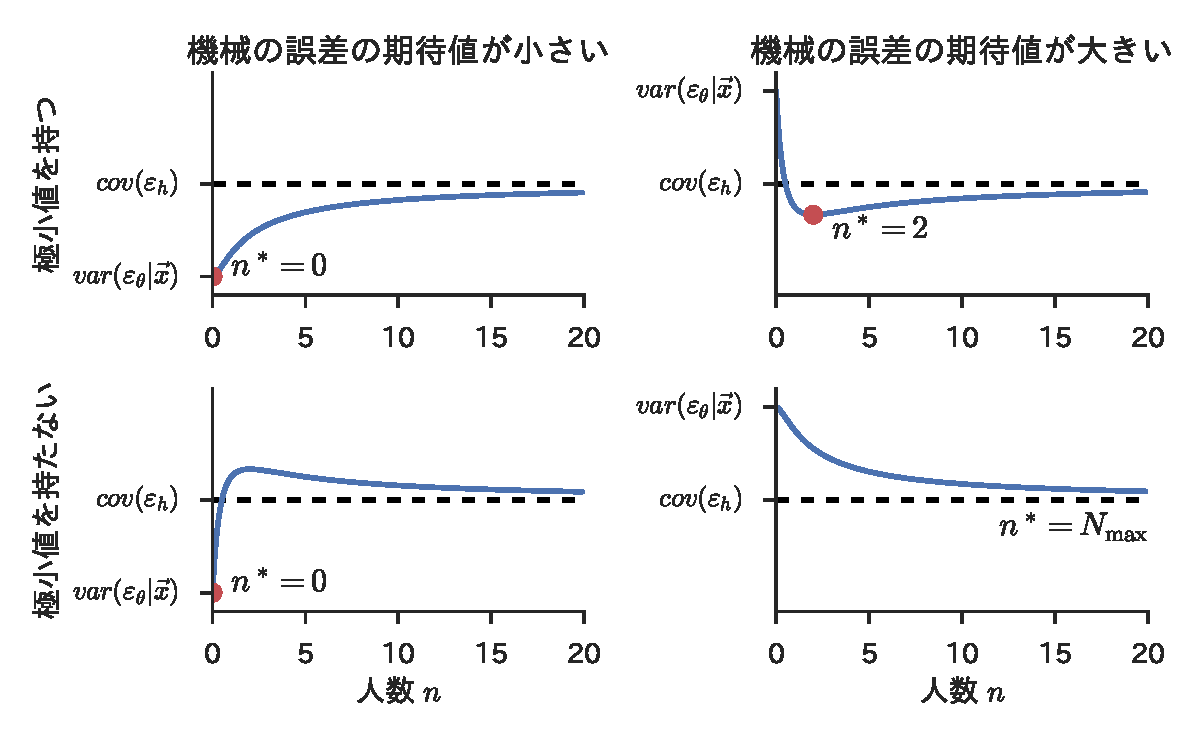
\includegraphics[width=\columnwidth]{slide-ensemble_graph.pdf}
      \caption{アンサンブルの二乗誤差の期待値と人数$n$の関係}
    \end{figure}
  \end{column}
\end{columns}
\end{frame}
%%%%%%%%%%%%%%%%%%%%%%%%%%%%%%%%%%%%%%%%

\section{実験}

\subsection{実験の目的}

%%%%%%%%%%%%%%%%%%%%%%%%%%%%%%%%%%%%%%%%
\begin{frame}{実験の目的}
\begin{block}{モデルの検証}
  \begin{itemize}
    \item 分布の分散を二乗誤差の期待値とみなせるといった仮定が現実の問題でも満たされるか検証する
  \end{itemize}
\end{block}
\begin{block}{実問題における予測精度の確認}
  \begin{itemize}
    \item $\varh$,$\covh$,$\covmh$の真の値を実際に知ることはできず,過去のサンプルから推定するしかない
    \item サンプル外で,推定したパラメータの値の通りに振る舞うとは限らない
  \end{itemize}
\end{block}
\begin{block}{提案したアンサンブル法の振る舞いの観察}
  \begin{itemize}
    \item 過去にないパターンが与えられた時に人間による予測を用いるという仮説の検証
    \item 2008年のリーマンショックを用いる
  \end{itemize}
\end{block}
\end{frame}
%%%%%%%%%%%%%%%%%%%%%%%%%%%%%%%%%%%%%%%%

\subsection{実験の方法}

%%%%%%%%%%%%%%%%%%%%%%%%%%%%%%%%%%%%%%%%
\begin{frame}{データ}
\begin{columns}
  \begin{column}{0.6\textwidth}
    \begin{block}{予測対象: インフレに関する4つの指標}
      \begin{itemize}
        \item 消費者物価指数 (CPI), Core CPI (1957〜)
        \item 個人消費支出 (PCE), Core PCE (1959〜)
      \end{itemize}
    \end{block}
    \begin{block}{人間の予測: 経済予測のサーベイ調査}
      \begin{itemize}
        \item Livingston survey (LIV)
        \begin{itemize}
          \item 1946年から6ヶ月ごと
          \item CPI のみ,6ヶ月後と12ヶ月後の予測
        \end{itemize}
        \item Survey of Professional Forecasts (SPF)
        \begin{itemize}
          \item 1981年から四半期ごと
          \item 全ての指標,1年後の予測のみ
        \end{itemize}
      \end{itemize}
    \end{block}
  \end{column}
  \begin{column}{0.4\textwidth}
    \begin{figure}
      \centering
      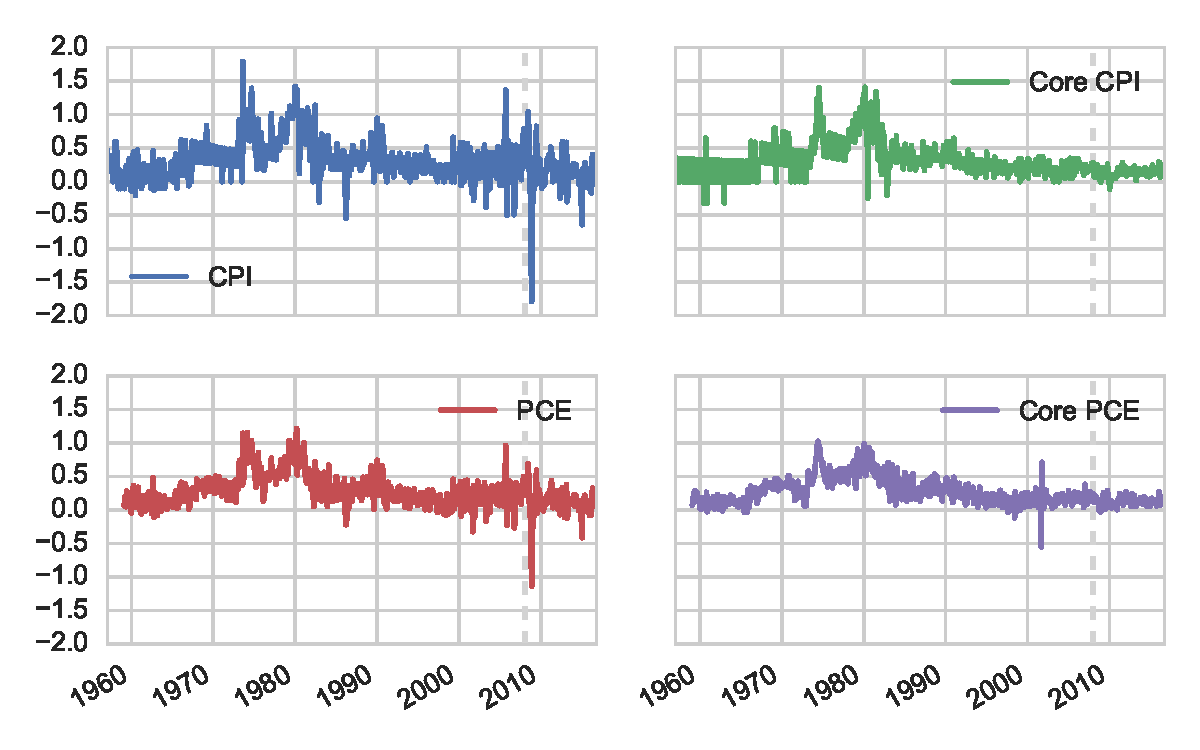
\includegraphics[width=\columnwidth]{slide-series.pdf}\\
      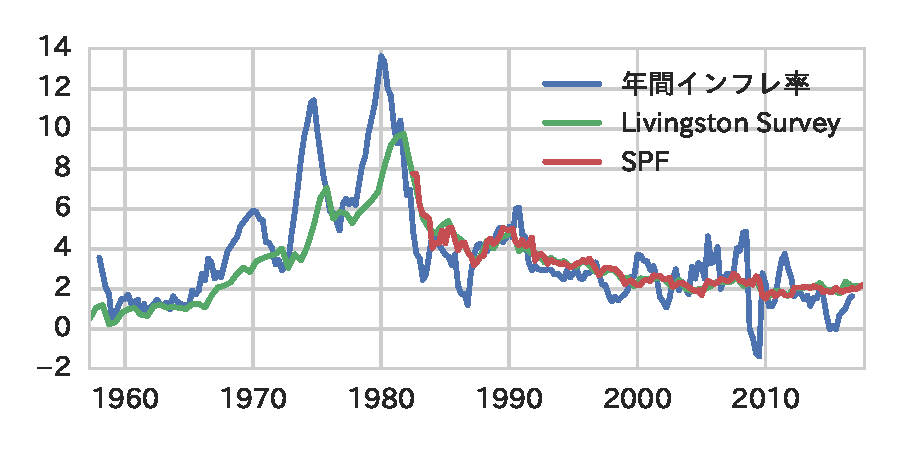
\includegraphics[width=\columnwidth]{slide-surveys.pdf}
    \end{figure}
  \end{column}
\end{columns}
\end{frame}
%%%%%%%%%%%%%%%%%%%%%%%%%%%%%%%%%%%%%%%%

%%%%%%%%%%%%%%%%%%%%%%%%%%%%%%%%%%%%%%%%
\begin{frame}{予測手法}
\begin{block}{ベンチマーク~\cite{Ang2007}}
  \begin{itemize}
    \item 従来の時系列解析の手法より,自己回帰移動平均モデル ARMA(1,1)
  \end{itemize}
\end{block}
\begin{block}{機械}
  \begin{itemize}
    \item 再帰ニューラルネットワーク (RNN)
    \begin{itemize}
      \item 入力: 過去12ヶ月の変化 / 出力: 目的の値の離散確率分布
    \end{itemize}
  \end{itemize}
\end{block}
\begin{block}{人間}
  \begin{itemize}
    \item LIV と SPF の各サーベイ
    \begin{itemize}
      \item 人数を統一するため各調査からランダムに5人をサンプルし,その平均値を取る
    \end{itemize}
  \end{itemize}
\end{block}
\begin{block}{提案手法}
  \begin{itemize}
    \item 機械 (RNN) と人間 (LIV, SPF) の組み合わせにより構成
  \end{itemize}
\end{block}
\end{frame}
%%%%%%%%%%%%%%%%%%%%%%%%%%%%%%%%%%%%%%%%

%%%%%%%%%%%%%%%%%%%%%%%%%%%%%%%%%%%%%%%%
\begin{frame}{評価方法}
\begin{block}{データセットの分割}
  \begin{itemize}
    \item 2008年以前を訓練セット,それ以降をテストセットとする
    \begin{itemize}
      \item 比較のため,CPIのみ1998年を境界とした場合も作成
    \end{itemize}
    \item 評価にはテストセットのみを用いる
    \begin{itemize}
      \item モデルの作成やパラメータの推定にはテストセットは用いない
    \end{itemize}
  \end{itemize}
\end{block}
\begin{block}{予測精度の評価指標}
  \begin{itemize}
    \item Root Mean Squared Error (RMSE) を用いる
    \begin{equation}
      \textstyle
      \RMSE(\bm{\hat{y}}) = \sqrt{\frac{1}{M}\sum_{i=1}^{M}(y_i - \hat{y}_i)}
      \nonumber
    \end{equation}
    \item ベンチマークの ARMA(1,1) のRMSEを1とした相対値を示す
  \end{itemize}
\end{block}
\end{frame}
%%%%%%%%%%%%%%%%%%%%%%%%%%%%%%%%%%%%%%%%

\section{結果}

\subsection{モデルの検証}

%%%%%%%%%%%%%%%%%%%%%%%%%%%%%%%%%%%%%%%%
\begin{frame}{モデルの検証(分布の分散と二乗誤差の関係)}
\begin{columns}
  \begin{column}{0.4\textwidth}
    \begin{block}{仮定}
      機械が出力した分布の分散を二乗誤差の期待値とみなせる
    \end{block}
    \begin{alertblock}{結果}
      バラつきは大きいが,おおよそ原点を通る傾き1の直線に沿って分布していた
    \end{alertblock}
  \end{column}
  \begin{column}{0.6\textwidth}
    \begin{figure}
      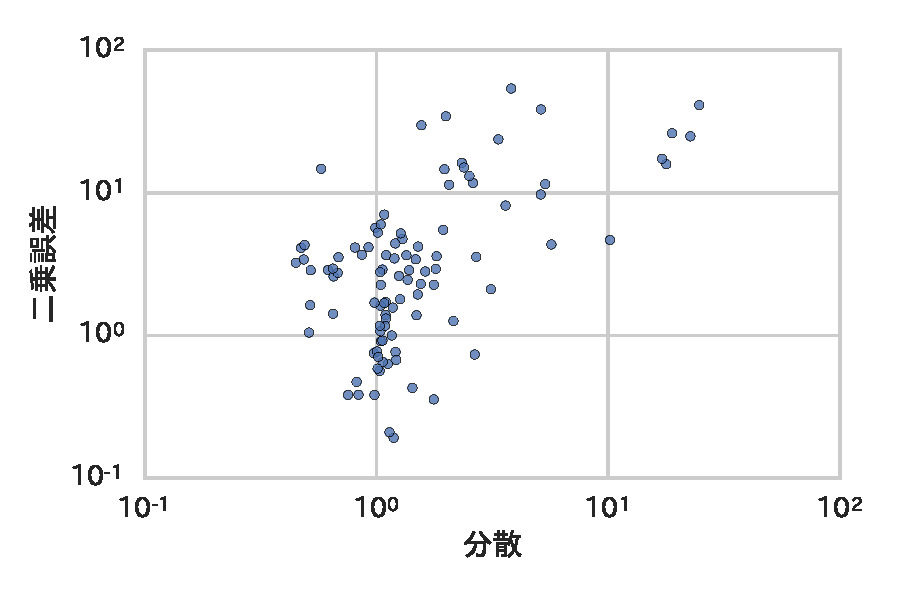
\includegraphics[width=\columnwidth]{slide-var_sqerr.pdf}
      \caption{テストセットにおける分布の分散と二乗誤差の関係 (CPI-LIV)}
    \end{figure}
  \end{column}
\end{columns}
\end{frame}
%%%%%%%%%%%%%%%%%%%%%%%%%%%%%%%%%%%%%%%%

\subsection{予測精度}

%%%%%%%%%%%%%%%%%%%%%%%%%%%%%%%%%%%%%%%%
\begin{frame}{予測精度}
\begin{table}
  \caption{相対RMSE}
  \begin{center}
    \small
    \begin{tabular}{lrrrrrrr}
\toprule
{} &  CPI-LIV &  CPI-SPF &  CoreCPI &    PCE &  CorePCE &  CPI-6M &  CPI-1998 \\
\midrule
ベンチマーク&    1.000 &    1.000 &    1.000 &  1.000 &    1.000 &   1.000 &     1.000 \\
機械      &    0.889 &    0.889 &    0.788 &  0.933 &    0.842 &   1.010 &     0.941 \\
人間      &    0.704 &\alert{0.736}&\alert{0.767}&\alert{0.711}&    0.848 &   0.939 &     0.940 \\
提案手法   &\alert{0.689}&\alert{0.736}&\alert{0.767}&  0.724 &\alert{0.827}&\alert{0.931} &\alert{0.755} \\
\bottomrule
\end{tabular}

  \end{center}
\end{table}
\begin{alertblock}{結果}
  \begin{itemize}
    \item \alert{提案手法は7つのうち4つで最も精度が高く,2つで既存手法と同じになった}
    \item CPI-SPF と CoreCPI では提案手法は人間による予測のみを用いた
  \end{itemize}
\end{alertblock}
\end{frame}
%%%%%%%%%%%%%%%%%%%%%%%%%%%%%%%%%%%%%%%%

\subsection{提案手法の振る舞い}

%%%%%%%%%%%%%%%%%%%%%%%%%%%%%%%%%%%%%%%%
\begin{frame}{提案手法の振る舞い}
\begin{columns}
  \begin{column}{0.4\textwidth}
    \begin{block}{想定シナリオ}
      過去にない系列が機械に与えられたとき人間による予測を用いる
    \end{block}
    \begin{alertblock}{結果}
      \alert{2008年9月のリーマンショック後,機械の誤差が大きいとき人間による予測をうまく利用していた}
    \end{alertblock}
  \end{column}
  \begin{column}{0.6\textwidth}
    \begin{figure}
      \centering
      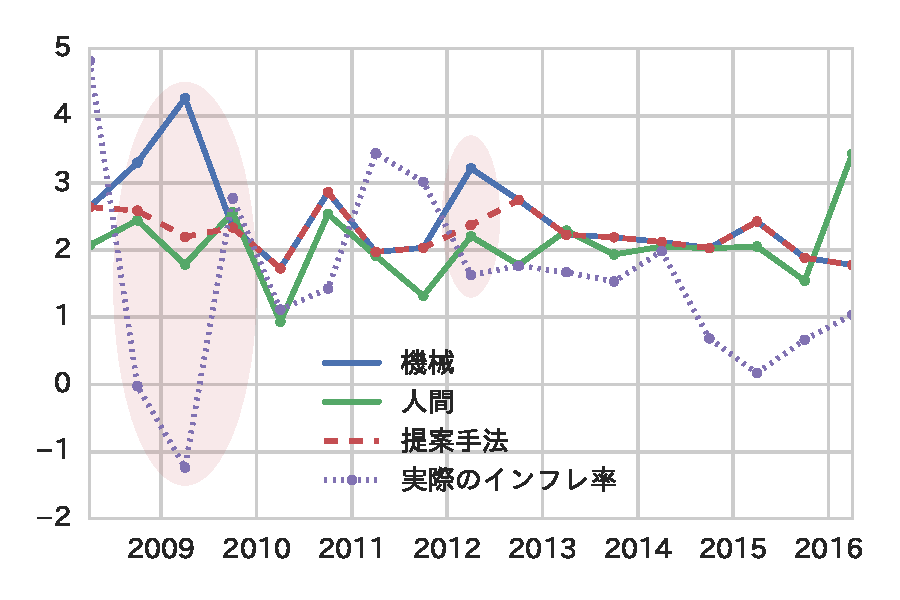
\includegraphics[width=\columnwidth]{slide-behavior.pdf}
      \caption{テストセットでの年間インフレ率予測 (CPI-LIV)}
    \end{figure}
  \end{column}
\end{columns}
\end{frame}
%%%%%%%%%%%%%%%%%%%%%%%%%%%%%%%%%%%%%%%%

\section{考察}

\subsection{提案手法の適用範囲}

%%%%%%%%%%%%%%%%%%%%%%%%%%%%%%%%%%%%%%%%
\begin{frame}{Human-Machine Ensemble Method の適用範囲}
\begin{block}{Human-Machine Ensemble を有効に使う条件}
  \begin{enumerate}
    \item 予測対象は数値など誤差を定義できるものである
    \item 機械が入力に応じた誤差の期待値を出力できる
    \item 人間の母集団について$\varh$,$\covh$が推定できる
    \item 機械の方が良い場合もあれば,人間の方が良い場合もある
    \begin{itemize}
      \item 人間と機械の多様性が人間同士の多様性よりも大きい ($\covmh < \covh$)
    \end{itemize}
  \end{enumerate}
\end{block}
\begin{table}
  \caption{各アンサンブルにおけるパラメータ.青字は$\covmh < \covh$が不成立}
  \begin{center}
    \small
    \begin{tabular}{lrrrrrrr}
\toprule
{} &  CPI-LIV &  CPI-SPF &  CoreCPI &    PCE &  CorePCE &  CPI-6M &  CPI-1998 \\
\midrule
$\covh$  &    1.846 &    0.873 &    0.455 &  0.450 &    0.168 &   0.652 &     1.924 \\
$\covmh$ &    1.772 &\structure{1.096}&\structure{0.668}&\structure{0.510}&    0.056 &   0.497 &     1.821 \\
\bottomrule
\end{tabular}

  \end{center}
\end{table}
\end{frame}
%%%%%%%%%%%%%%%%%%%%%%%%%%%%%%%%%%%%%%%%

\subsection{今後の課題}

%%%%%%%%%%%%%%%%%%%%%%%%%%%%%%%%%%%%%%%%
\begin{frame}{今後の課題}
\begin{block}{提案手法の応用}
  実際には,人間の予測にデータの蓄積がある専門家の予測が使えるとは限らない\\
  \structure{$\to$} 人間の予測にクラウドソーシングを用いる
  \begin{itemize}
    \item 一般人を対象にした Michigan survey もLIVやSPFと同程度の予測精度がある
    \item EMアルゴリズム等を用いてパラメータ$\varh$,$\covh$を推定する必要がある
  \end{itemize}
\end{block}
\begin{block}{提案手法の拡張}
  今回は,同一のパラメータに従う複数の人間と一つの機械の予測値を単純平均した\\
  \structure{$\to$} 組み合わせ方を拡張してより正確な予測を目指す
  \begin{itemize}
    \item 機械の数も可変にする
    \item 人間を経済学者と金融アナリストなど複数のタイプに分ける
    \item 単純平均以外の集約方法を用いる
  \end{itemize}
\end{block}
\end{frame}
%%%%%%%%%%%%%%%%%%%%%%%%%%%%%%%%%%%%%%%%

\section{まとめ}

%%%%%%%%%%%%%%%%%%%%%%%%%%%%%%%%%%%%%%%%
\begin{frame}{まとめ}
\begin{block}{研究の目的}
  人間と機械の予測をうまく組み合わせることで,より正確な経済予測を行う
\end{block}
\begin{alertblock}{本研究の貢献}
  \begin{enumerate}
    \item 人間と機械の予測方法の違いを反映したモデル化と,最適な組み合わせ方の考案
    \begin{itemize}
      \item 事後分布を用いて入力ごとに誤差の期待値が異なる予測をモデル化した
      \item そのモデルの元で誤差の期待値を最小化する人数を求める方法を提示した
    \end{itemize}
    \medskip
    \item 考案したアンサンブル法を用いた経済予測の実装と評価
    \begin{itemize}
      \item 実際のインフレ予測に提案したモデル・手法が適用可能であることを示した
      \item 7つのデータ中4つで予測精度の改善を確認した
    \end{itemize}
  \end{enumerate}
\end{alertblock}
\end{frame}
%%%%%%%%%%%%%%%%%%%%%%%%%%%%%%%%%%%%%%%%

\section*{参考文献}

%%%%%%%%%%%%%%%%%%%%%%%%%%%%%%%%%%%%%%%%
\begin{frame}{参考文献}
\bibliographystyle{kuissort}
\bibliography{../paper/master-thesis.bib}
\end{frame}
%%%%%%%%%%%%%%%%%%%%%%%%%%%%%%%%%%%%%%%%

\appendix

%%%%%%%%%%%%%%%%%%%%%%%%%%%%%%%%%%%%%%%%
\begin{frame}{パラメータの推定}
\begin{align*}
  \varh &= \frac{1}{N}\sum_{i=1}^N\var(\varepsilon_{h_i}) \\
  \covh &= \frac{1}{N(N - 1)}\sum_{i=1}^N\sum_{j \neq i}\cov(\varepsilon_{h_i}, \varepsilon_{h_j}) \\
  \covmh &= \frac{1}{N}\sum_{i=1}^N\cov(\varepsilon_\theta, \varepsilon_{h_i})
\end{align*}
\begin{itemize}
  \item $\var(\varepsilon_{h_i})$: 予測者$i$の予測値の分散
  \item $\cov(\varepsilon_{h_i}, \varepsilon_{h_j})$: 予測者$i$と$j$の誤差の共分散
  \item $\cov(\varepsilon_{\theta}, \varepsilon_{h_i})$: 予測器$\theta$と予測者$i$の誤差の共分散
\end{itemize}
\end{frame}
%%%%%%%%%%%%%%%%%%%%%%%%%%%%%%%%%%%%%%%%

%%%%%%%%%%%%%%%%%%%%%%%%%%%%%%%%%%%%%%%%
\begin{frame}{実験で使用した RNN のアーキテクチャ}
\begin{columns}
  \begin{column}{0.5\textwidth}
    \begin{itemize}
      \item ``None'' にはミニバッチのサンプル数32が入る
      \item 出力層の次元``28''は12ヶ月後のCPIを予測する場合
    \end{itemize}
  \end{column}
  \begin{column}{0.5\textwidth}
    \begin{figure}
      \centering
      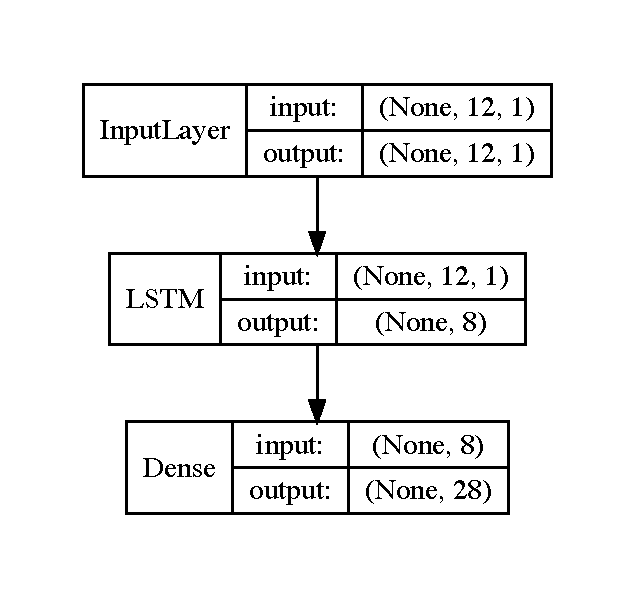
\includegraphics[width=\columnwidth]{experiment-machine_model}
      % \caption{}
    \end{figure}
  \end{column}
\end{columns}
\end{frame}
%%%%%%%%%%%%%%%%%%%%%%%%%%%%%%%%%%%%%%%%

%%%%%%%%%%%%%%%%%%%%%%%%%%%%%%%%%%%%%%%%
\begin{frame}{実験で使用した RNN の出力層のラベル}
\begin{itemize}
  \item 訓練データにおける最小値 (min) から最大値 (max) までを step の値で区切る
  \item 出力層の活性化関数にソフトマックス関数を用いて離散確率分布を出力させる
\end{itemize}
\begin{table}
  \caption{出力層におけるラベルの最小値と最大値,個数,ラベル間の値の差}
  \begin{center}
    \small
    \begin{tabular}{lrrrrr}
\toprule
{} &  CPI(12M) &  CPI(6M) &  CoreCPI &   PCE &  CorePCE \\
\midrule
min  &       0.1 &     -0.4 &       0.7 &   0.5 &       0.9 \\
max  &      13.6 &      7.4 &      12.7 &  11.0 &       9.9 \\
size &        28 &       27 &        25 &    22 &        19 \\
step &       0.5 &      0.3 &       0.5 &   0.5 &       0.5 \\
\bottomrule
\end{tabular}

  \end{center}
\end{table}
\end{frame}
%%%%%%%%%%%%%%%%%%%%%%%%%%%%%%%%%%%%%%%%

%%%%%%%%%%%%%%%%%%%%%%%%%%%%%%%%%%%%%%%%
\begin{frame}{実験で使用したアンサンブルの種類}
\begin{table}
  \caption{実験で使用したアンサンブルの種類}
  \begin{center}
    \small
    \begin{tabular}{llllllll}
\toprule
{} & CPI-LIV & CPI-SPF &   CoreCPI &   PCE &   CorePCE & CPI-6M & CPI-1998 \\
\midrule
target index   &     CPI &     CPI &  CoreCPI &   PCE &  CorePCE &    CPI &      CPI \\
survey source   &     LIV &     SPF &       SPF &   SPF &       SPF &    LIV &      LIV \\
forecast period &     12M &     12M &       12M &   12M &       12M &     6M &      12M \\
dataset boundary &    2008 &    2008 &      2008 &  2008 &      2008 &   2008 &     1998 \\
\bottomrule
\end{tabular}

  \end{center}
\end{table}
\end{frame}
%%%%%%%%%%%%%%%%%%%%%%%%%%%%%%%%%%%%%%%%

%%%%%%%%%%%%%%%%%%%%%%%%%%%%%%%%%%%%%%%%
\begin{frame}{モデルの検証(人間の予測誤差の分布)}
\begin{columns}
  \begin{column}{0.55\textwidth}
    \begin{block}{仮定}
      人間による予測値に偏りはないと仮定した
    \end{block}
    \begin{alertblock}{結果}
      0を中心に偏りなく分布している\\
      (LIV,SPFの平均値はそれぞれ$-0.40$,$0.37$)
    \end{alertblock}
  \end{column}
  \begin{column}{0.45\textwidth}
    \begin{figure}
      \centering
      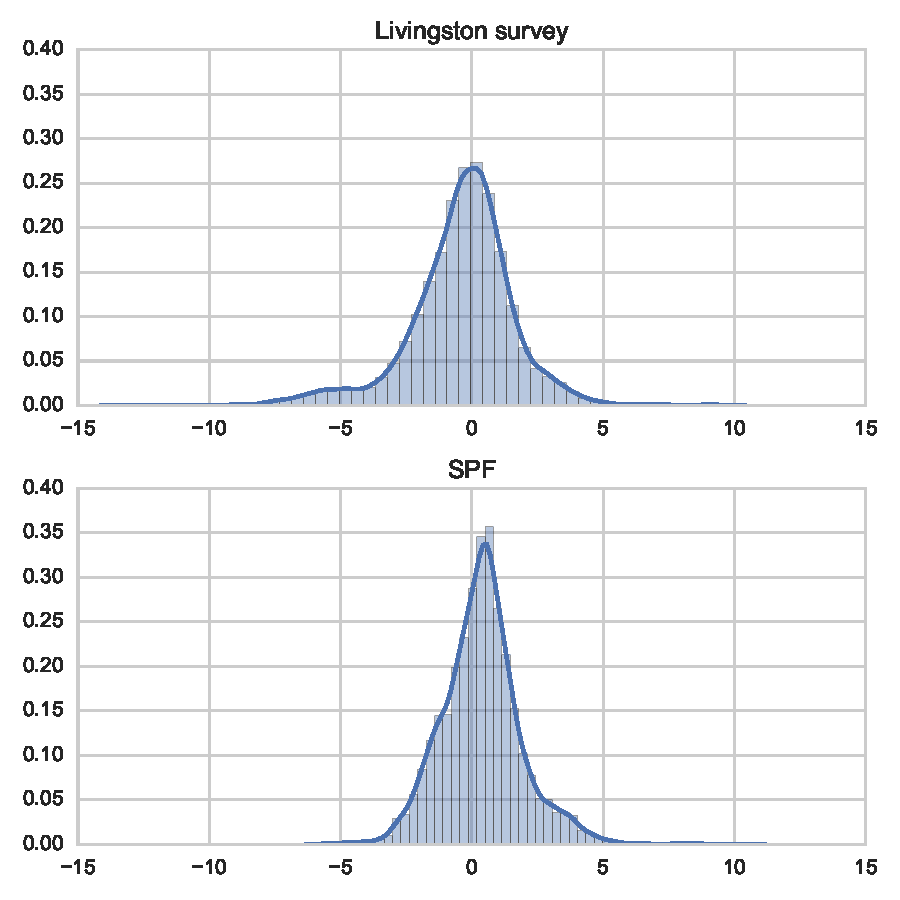
\includegraphics[width=\columnwidth]{results-error_distribution.pdf}
      % \caption{}
    \end{figure}
  \end{column}
\end{columns}
\end{frame}
%%%%%%%%%%%%%%%%%%%%%%%%%%%%%%%%%%%%%%%%

%%%%%%%%%%%%%%%%%%%%%%%%%%%%%%%%%%%%%%%%
\begin{frame}{ARMA(1,1) で正規化する前の RMSE}
\begin{table}
  \caption{絶対RMSE}
  \begin{center}
    \small
    \begin{tabular}{lrrrrrrr}
\toprule
{} &  CPI-LIV &  CPI-SPF &  CoreCPI &    PCE &  CorePCE &  CPI-6M &  CPI-1998 \\
\midrule
ベンチマーク&    2.234 &    2.234 &    0.603 &  1.698 &    0.546 &   1.360 &     1.740 \\
機械      &    1.985 &    1.985 &    0.475 &  1.585 &    0.460 &   1.374 &     1.637 \\
人間      &    1.572 &\alert{1.644}&\alert{0.462}&\alert{1.207}&    0.463 &   1.277 &     1.635 \\
提案手法   &\alert{1.540}&\alert{1.644}&\alert{0.462}&  1.230 &\alert{0.451}&\alert{1.265}&\alert{1.314} \\
\bottomrule
\end{tabular}

  \end{center}
\end{table}
\end{frame}
%%%%%%%%%%%%%%%%%%%%%%%%%%%%%%%%%%%%%%%%

%%%%%%%%%%%%%%%%%%%%%%%%%%%%%%%%%%%%%%%%
\begin{frame}{提案手法の振る舞い(詳細)}
\begin{columns}
  \begin{column}{0.4\textwidth}
    左から
    \begin{itemize}
      \item 機械の二乗誤差
      \item 機械の出力した分布の分散
      \item 提案手法で用いられた人数$n$
      \item 提案手法の二乗誤差
    \end{itemize}
    \medskip
    式(\ref{eq: condition})が成り立たないため\\
    $n$が$0$か$5 (= N_{\max})$しか取れない
  \end{column}
  \begin{column}{0.6\textwidth}
    \begin{table}
      \begin{center}
        \scriptsize
        \begin{tabular}{lrrrr}
\toprule
{} &  machine error &  variance &  n &  ensemble error \\
\midrule
Jun 2008 &           4.74 &      1.53 &  0 &            4.74 \\
Dec 2008 &          11.06 &      2.15 &  5 &            6.81 \\
Jun 2009 &          30.23 &      2.81 &  5 &           11.80 \\
Dec 2009 &           0.19 &      1.63 &  0 &            0.19 \\
Jun 2010 &           0.38 &      0.90 &  0 &            0.38 \\
Dec 2010 &           2.06 &      1.72 &  0 &            2.06 \\
Jun 2011 &           2.16 &      1.15 &  0 &            2.16 \\
Dec 2011 &           0.96 &      1.22 &  0 &            0.96 \\
Jun 2012 &           2.51 &      2.12 &  5 &            0.55 \\
Dec 2012 &           0.96 &      1.65 &  0 &            0.96 \\
Jun 2013 &           0.31 &      1.35 &  0 &            0.31 \\
Dec 2013 &           0.43 &      1.33 &  0 &            0.43 \\
Jun 2014 &           0.02 &      1.28 &  0 &            0.02 \\
Dec 2014 &           1.81 &      1.21 &  0 &            1.81 \\
Jun 2015 &           5.08 &      1.45 &  0 &            5.08 \\
Dec 2015 &           1.49 &      1.07 &  0 &            1.49 \\
Jun 2016 &           0.55 &      0.96 &  0 &            0.55 \\
\bottomrule
\end{tabular}

      \end{center}
    \end{table}
  \end{column}
\end{columns}
\end{frame}
%%%%%%%%%%%%%%%%%%%%%%%%%%%%%%%%%%%%%%%%

%%%%%%%%%%%%%%%%%%%%%%%%%%%%%%%%%%%%%%%%
\begin{frame}{極小値を持つ場合の人工的な例}
\begin{table}
  \caption{$\varh = 3$, $\covh = 2$, $\covmh = 0$として生成したサンプル}
  \begin{center}
    \small
    \begin{tabular}{lrrr}
\toprule
{} & $\varepsilon_{h_1}$ & $\varepsilon_{h_2}$ & $\varepsilon_\theta$ \\
\midrule
0 &  0.1 &  1.0 &    1.7 \\
1 & -0.5 &  0.3 &    1.3 \\
2 & -2.1 & -2.5 & \alert{2.9} \\
3 & -0.3 &  2.5 &   -1.2 \\
4 & -2.4 & -3.3 & \alert{0.8} \\
5 & -0.4 &  0.1 &    2.6 \\
6 & -0.2 &  0.5 &    1.6 \\
7 &  1.6 &  1.0 &    0.7 \\
8 &  0.3 & -0.4 &   -0.9 \\
9 &  0.9 &  1.9 &    1.9 \\
\bottomrule
\end{tabular}

  \end{center}
\end{table}
\end{frame}
%%%%%%%%%%%%%%%%%%%%%%%%%%%%%%%%%%%%%%%%

\end{document}
